% !TEX root = paper.tex
% !TEX encoding = UTF-8 Unicode
% -*- coding: UTF-8; -*-
% vim: set fenc=utf-8
% !TEX spellcheck = en-US
%=================================================================
\section{Results}
\label{sec:results}
%=================================================================
%------------------------------%

\begin{figure}[t!]%%[p!]
	%\flushleft{\bf (A) \hspace{4.2cm} (B) \hspace{2cm} (C) \hspace{4cm} (D)\hspace{6cm}}
	\centering{{\bf a.} \hspace{1.6cm} {\bf b.} \hspace{1.6cm} {\bf c.} \hspace{1.6cm} {\bf d.} \hspace{1.6cm} {\bf e.}}
	\centering{\A\includegraphics[width=.9\linewidth]{CNS-saccade-8.png}}
	\centering{\B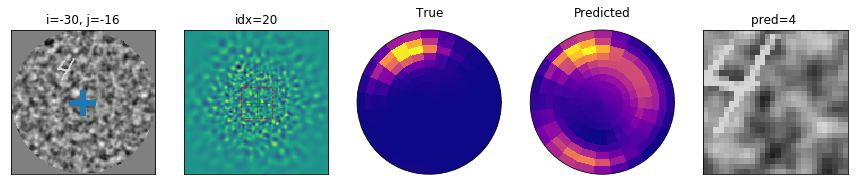
\includegraphics[width=.9\linewidth]{CNS-saccade-20.png}}
	\centering{\C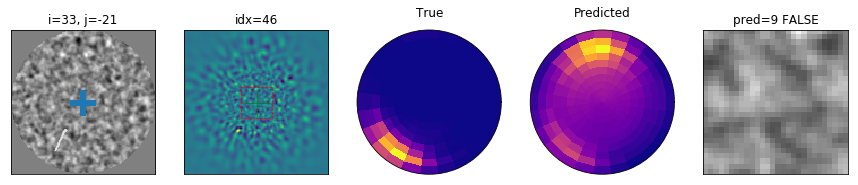
\includegraphics[width=.9\linewidth]{CNS-saccade-46.png}}
	\centering{\D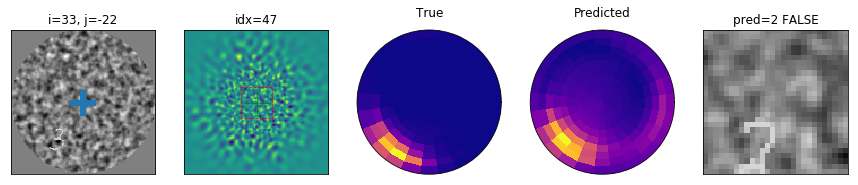
\includegraphics[width=.9\linewidth]{CNS-saccade-47.png}}
	\centering{\E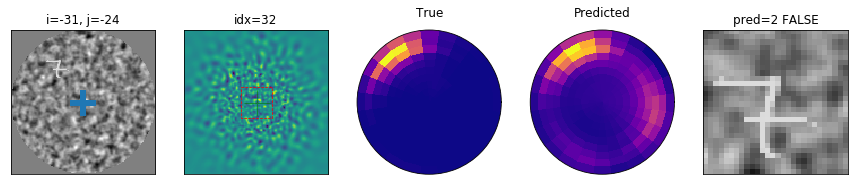
\includegraphics[width=.9\linewidth]{CNS-saccade-32.png}}		% \includegraphics[]{../../2019-07-15_CNS/figures/CNS-saccade-8.png} % TRUE
	\caption{
		{\A-- \E Active vision samples after training}. \A-- \B  classification success samples. \C-- \E classification failure samples. Digit contrast set to 0.7.  From left to right :
		{\bf a.} The initial 128$\times$128 visual display, with blue cross giving the center of gaze.  
		The visual input is retinotopically transformed and sent to the multi-layer neural network implementing the ``Where'' pathway. 
		{\bf b.} Magnified reconstruction of the  visual input, as it shows off from the primary visual features through an inverse log-polar transform. 
		{\bf c.-d.} Color-coded radial representation of the output accuracy maps, with dark violet for the lower accuracies, and yellow for the higher accuracies. The network output ('Predicted') is visually compared with the ground truth ('True'). %
		{\bf e.} $28 \times 28$ central snippet as extracted from the visual display after doing a saccade, with label prediction and success flag in the title. 
		\label{fig:saccades}}%
\end{figure}%

%%------------------------------%
%=================================================================
\subsection{Inferring the target label from active visual search}
%=================================================================
After training, the ``Where'' pathway is now capable to predict an accuracy map, whose maximal argument drives the eye toward a new viewpoint. There, a central snippet is extracted, that is processed through the ``What'' pathway, allowing to predict the digit's label. Examples of this simple open loop sequence are presented in figure \ref{fig:saccades}, when the digits contrast parameter is set to 0.7 and the digits eccentricity varies between 0 and 40 pixels. The presented examples correspond to strong eccentricity cases, when the target is hardly visible on the display (fig. \ref{fig:saccades}a), and almost invisible on the reconstructed input (fig. \ref{fig:saccades}b). The radial maps (fig. \ref{fig:saccades}c-d) respectively represent the actual and the predicted accuracy maps. The final focus is represented in fig. \ref{fig:saccades}e, with cases of classification success (fig. \ref{fig:saccades}A-B) and cases of classification failures (fig. \ref{fig:saccades}C-E).  
In the case of successful detection (fig. \ref{fig:saccades}A-B), the accuracy prediction is not perfect and the digit is not perfectly centered on the fovea. This ``close match'' however allows for a correct classification for the digit's pixels are fully present on the fovea. The case of fig. \ref{fig:saccades}B and \ref{fig:saccades}C
 is interesting for it shows two cases of a bimodal prediction, indicating that the network is capable of doing multiple detections at a single glance. The case of \ref{fig:saccades}C corresponds to a false detection, with the true target detected still, though with a lower intensity. The case of fig. \ref{fig:saccades}D is a ``close match'' detection that is not precise enough to correctly center the visual target. Not every pixel of the digit being visible on the fovea, the label prediction is mistaken.
The last failure case (fig. \ref{fig:saccades}E) corresponds to a correct detection that is harmed by a wrong label prediction, only due to the ``What'' classifier inherent error rate.  
% We observed that either the detection of the object's position was correct, thus allowing a classification proportional to the accuracy of the ``what'' pathway, either that the predicted accuracy map was wrong and generated a wrong classification with an accuracy at chance level. 


%: see Figure~\ref{fig:results}
\begin{figure}[t!]%%[p!]
	%\flushleft{\bf (A) \hspace{4.2cm} (B) \hspace{2cm} (C) \hspace{4cm} (D)\hspace{6cm}}
	\centering{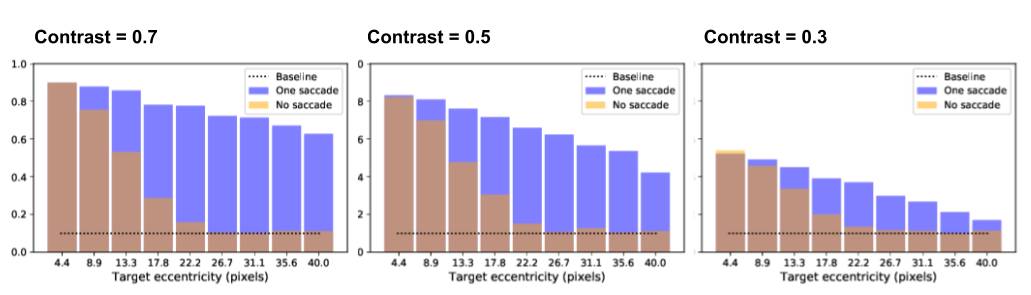
\includegraphics[width=\linewidth]{fig-results-contrast.png}}
	% \includegraphics[]{../../2019-07-15_CNS/figures/CNS-saccade-8.png} % TRUE
	\caption{
		{\bf Effect of contrast and target eccentricity.} %
		The active vision agent is tested for different target eccentricities (in pixels) and different contrasts to estimate a final classification rate. Orange bars: accuracy of a central classifier ('No saccade') with respect to the target's eccentricity, averaged over 1,000 trials per eccentricity scale. Blue bars: Final classification rate after one saccade, as predicted by the ``Where'' pathway. % \if 0\ICANN{\color{blue} TODO: show three levels of noise Low (0.5) median (1.2) high (2). TODO: compare with Accuracy max (knowing the position)}\fi
		\label{fig:results}}%
\end{figure}%


%The result of Figure~\ref{fig:results}-D, correspond to a SNR of $0.7$ and we replicated the result for SNRs of $0.3$ and $0.5$. First, we re-iterated for each SNR the whole process, first by learning the ``what'' pathway, then the accuracy maps and finally the ``where'' pathway. 


To test the robustness of our framework,the same experiment was repeated at different signal-to-noise ratios (SNR) of the input images. Both pathways being interdependent, it is crucial to disentangle the relative effect of of both sources of errors in the final accuracy. By manipulating the SNR and the target eccentricity, one can precisely monitor the network detection and recognition capabilities, with a detection task ranging from `easy'' (small shift, strong contrast) to ``almost impossible'' (large shift, low contrast). The  digit recognition capability is systematically evaluated in Figure~\ref{fig:results} for different eccentricities and different contrasts. 
%in simulation as the average accuracy obtained at the landing of the predicted saccade (see). For each different visual display (a different digit at a different position with a different noise clutter), a retinocentric visual input is processed (figure \ref{fig:results}-A), providing a predicted accuracy map (figure \ref{fig:results}-B) that can be compared to the actual future accuracy. Then, a saccade is carried out based on the most probable position as computed from the predicted accuracy map (figure \ref{fig:results}-C), and the final accuracy is computed from the ``what'' pathway using LeNet model.
For 3 target contrasts conditions ranging from 0.3 to 0.7, and 10 different eccentricities ranging from 4 to 40 pixels, the final accuracy is tested on $1,000$ trials both on the initial central snippet and the final central snippet (read at the landing of the first saccade). 
The orange bars provide the initial classification rate (without saccade) and the blue bars provide the final classification rate (after one saccade) -- see figure \ref{fig:results}.  As expected, the accuracy decreases with the eccentricity, for the targets become less and less visible in the periphery. The decrease is rapid in the central classifier case: the accuracy drops to the baseline level
at approximately $20$ pixels away from the center of gaze. The saccade-driven accuracy has a much wider range, with a slow decrease up to the border of the visual display (40 pixels away from the center). 
When varying the target contrast, the initial accuracy profile is scaled by the reference accuracy (obtained with a central target), whose values are approximately $53\%$, $82\%$ and $92\%$ for SNRs of $0.3$, $0.5$ and $0.7$. The saccade-driven accuracy profile is also similar at the different SNRs values, yet with the scaling imposed by the ``what'' pathway. This contrast-dependent scaling shows the robustness of our framework to the different factors of difficulty.

The high contrast case (fig.~\ref{fig:results}A) provides the greatest difference between the two profiles, with an accuracy approaching 0.9 at the center and 0.6 at the periphery. This allows to recognize digits after one saccade in a majority of cases, up to the border of the image, from a very scarce peripheral information. This full covering of the 128$\times$128 image range is done at a much lesser cost than would be done by a systematic image scan, as in classic computer vision. With decreasing target contrast, a general decrease of the accuracy is observed, both at the center and at the periphery, with about 10\% decrease with a contrast of 0.5, and 40\% decrease with a contrast of 0.3. In addition, the proportion of false detections also increases with contrast decrease. At 40 pixels away from the center, the false detection rate is approximately 30\% for a contrast of 0.7, 50\% for a contrast of 0.5 and 70\% for a contrast of 0.3 (with a recognition close to the baseline at the periphery in that case). The accuracy gain (difference between the initial and the final accuracy) is maximal for eccentricities ranging from 15 to 30 pixels. This optimal range reflects a peripheral region around the fovea where the target detection is possible, but not its identification. The visual agent knows \emph{where} the target is, without exactly knowing \emph{what} it is. 
More generally, this accuracy difference, that quantifies the benefit of active inference with respect to a central prior, can be interpreted as an approximation of the information gain provided by the ``Where'' pathway\footnote{with the true label log-posterior seen as a sample of the posterior entropy -- see eq.(\ref{eq:IG}).}.
% energy consumption

%The benefit of active inference can be enhanced by doing several saccades.   

%As our saccade selection algorithm may implement the essential operations done in the ``Where'' pathway, the central classifier may also reflect the response of the ``What'' pathway, giving the potential category of the digit. 

When both pathways are considered working in parallel, it is moreover possible to compare the two accuracy estimates to choose the most appropriate action: it may be that the accuracy is higher in the ``What'' pathway when the target is close to the center of gaze. In that case no saccade should be produced, and a categorical response should be given instead. The decision frontier lies 2-3 pixels away from the center, %between the first and the second spatial scale, 
allowing to pursue micro-saccades in the close vicinity of the target, in order to improve the centering and thus the classification accuracy. 
In the other decision case, the ''What'' accuracy can still be considered helpful to update the ``Where'' accuracy. 
When extending our framework to several saccades, this would allow in particular to ``explain away" the current position of the fixation and the neighboring ones. Such heuristic gives a principled formulation of the inhibition of return mechanism which is an important aspect for modeling saccades~\citep{Itti01}. In particular, we predict that such a mechanism is dependent on the class of inputs, and would be different for searching for faces as compared to digits. 

\subsection{Quantitative role of parameters}
%: effect of contrast


%: scanning of other parameters
In addition, we controlled that these results are robust to changes in an individual experimental or network parameters from the default parameters (see Figure~\ref{fig:params}). From the scan of each of these parameters, the following observations were remarkable. First we verified that accuracy decreased when \texttt{noise} increased and while the bandwidth of the noise imported weakly, the spatial frequency of the noise was an important factor. In particular, final accuracy was worst for $\texttt{sf\_0} \approx 0.07$, that is when the characteristic textures elements were close to the characteristic size of the objects. Second, we saw that the dimension of the ``Where'' network was optimal for a dimensionality similar to that of the input but that this mattered weakly. The dimensionality of the log-polar map is more important. The analysis proved that an optimal accuracy was achieved when using a number of $24$ azimuthal directions. Indeed, a finer log-polar grid requires more epochs to converge and may result in an over-fitting phenomenon hindering the final accuracy. Such fine tuning of parameters may prove to be important in practical applications and to optimize the compromise between accuracy and compression. 
%=================================================================
%------------------------------%
%: see Figure~\ref{fig:params}
\begin{figure}[t!]%%[p!]
\centering{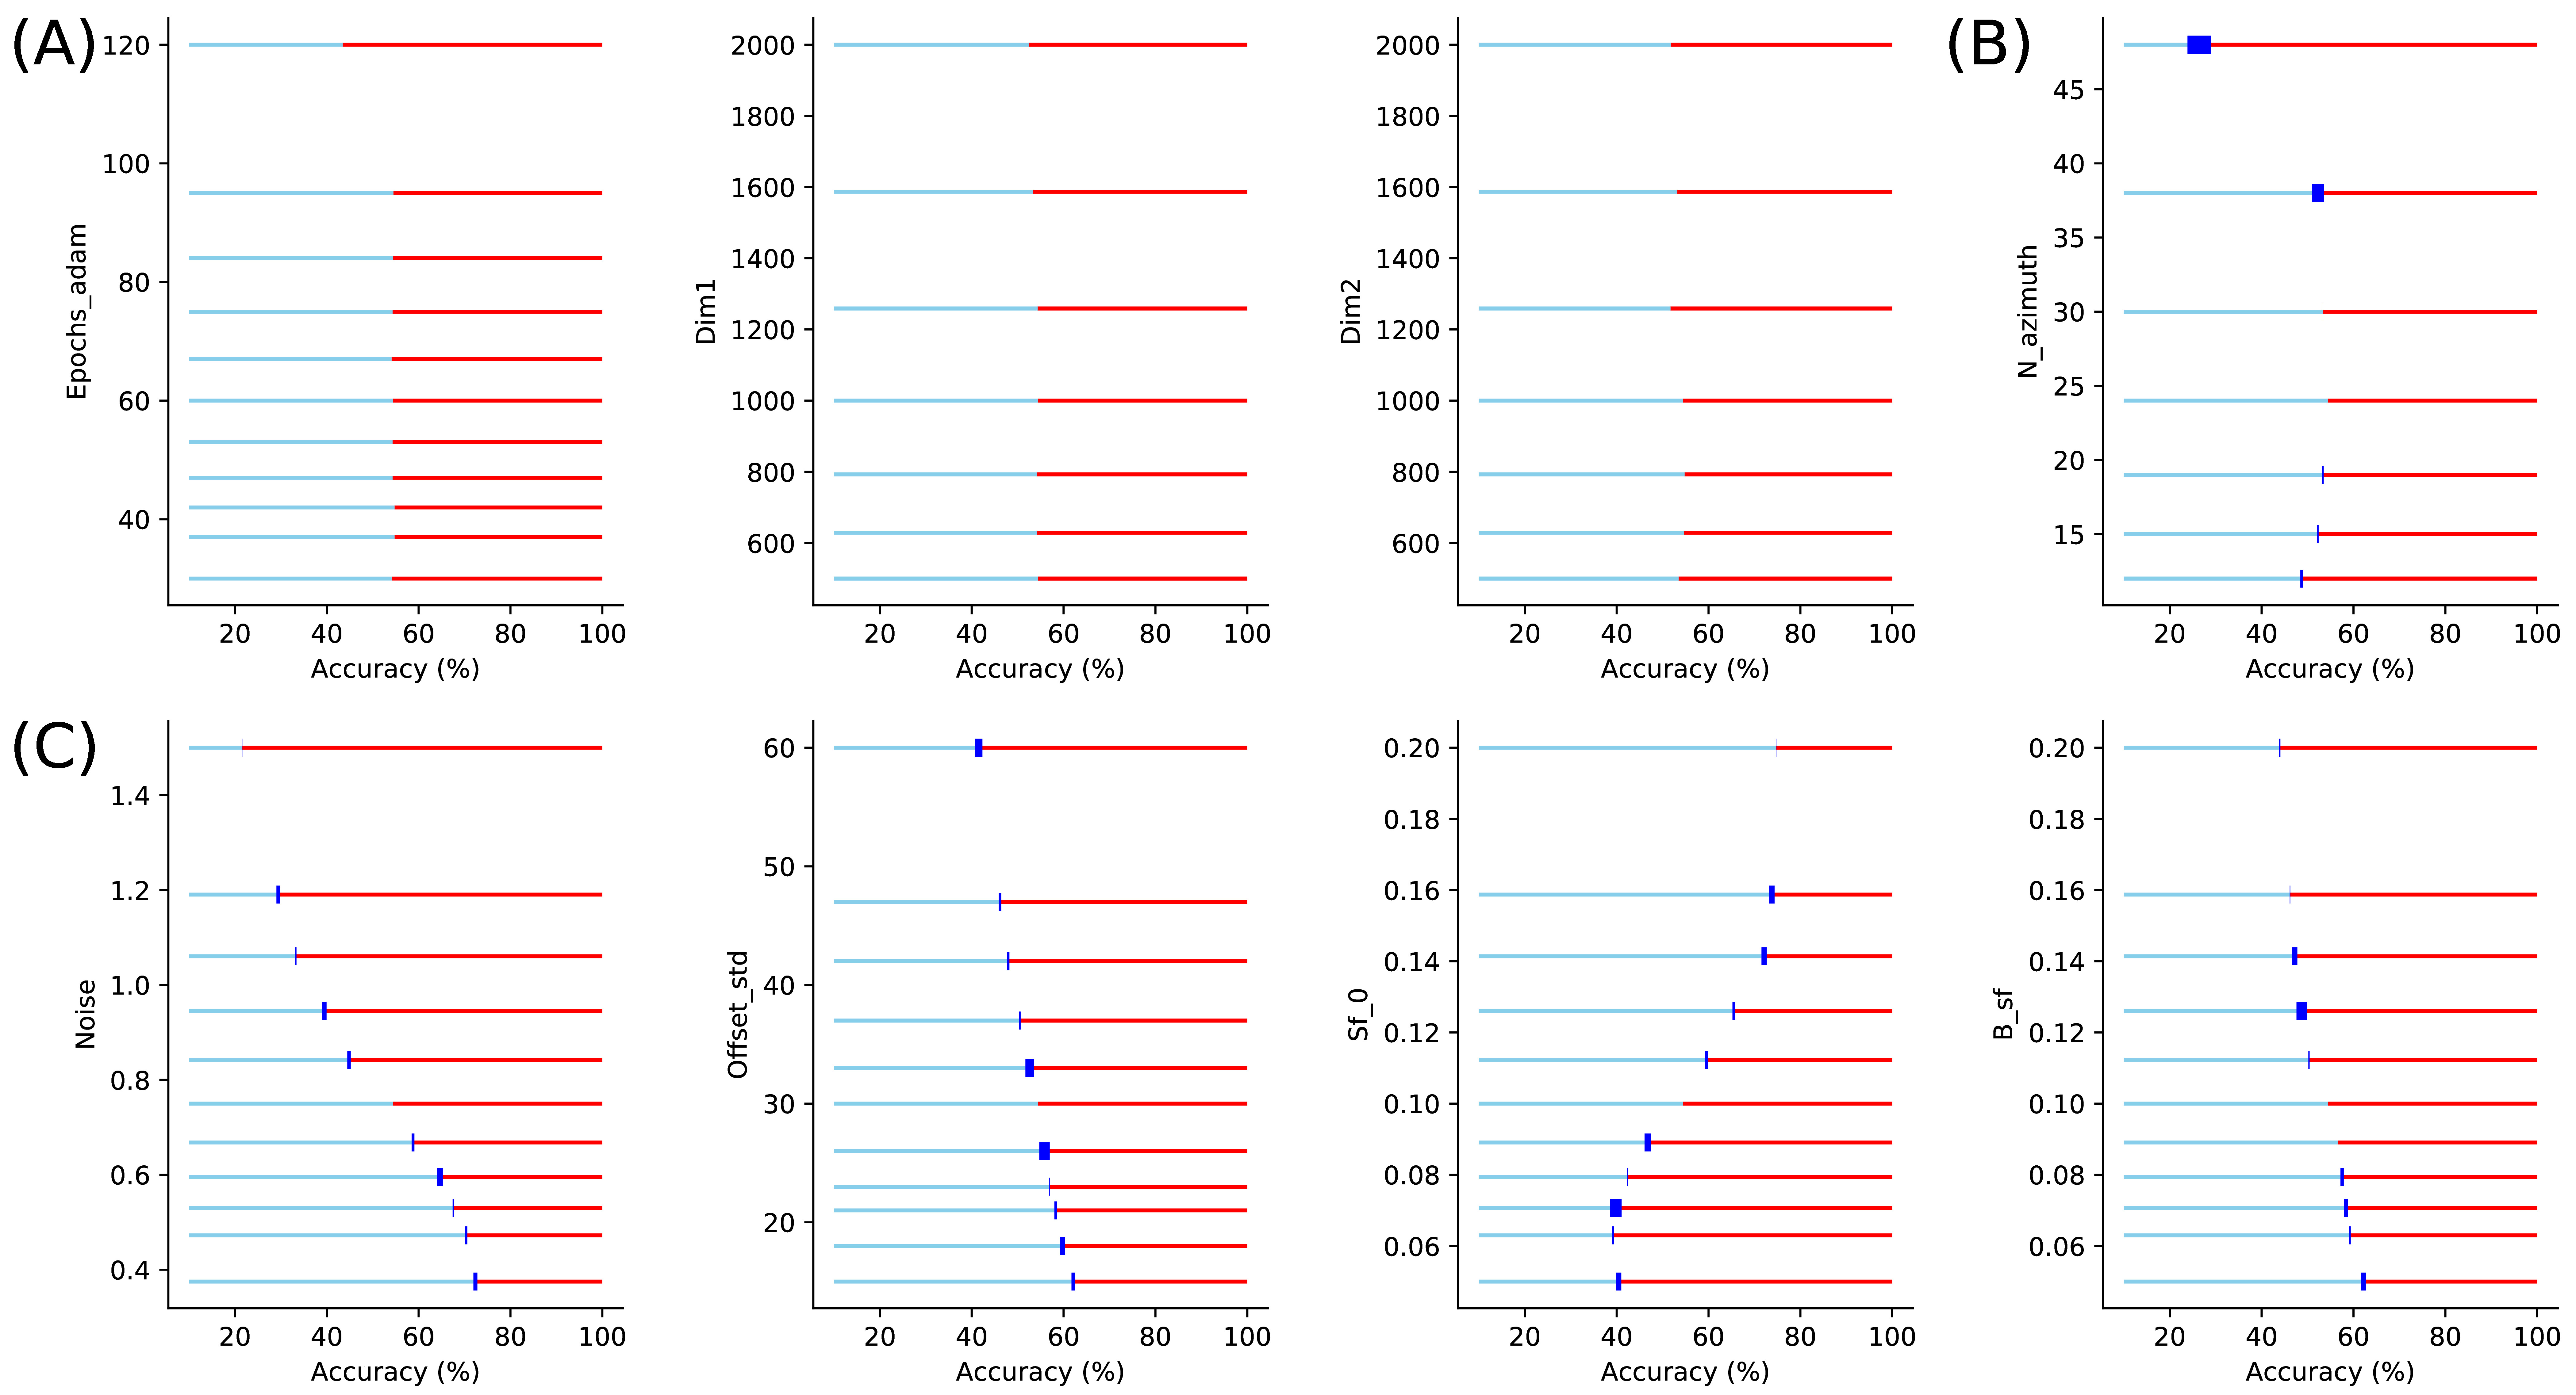
\includegraphics[width=\linewidth]{fig_params}}
\caption{
{\bf Quantitative role of parameters}: We show here variations of the average accuracy as a function of some free parameters of the model. All parameters of the presented model were tested, from the architecture of image generation, to the parameters of the neural network implementing the ``Where'' pathway (including meta-parameters of the learning paradigm). We show here the results which show the most significative impact on average accuracy. %
\A First, we tested some properties of the input, respectively from left to right: noise level (\texttt{noise}), mean spatial frequency of clutter \texttt{sf\_0} and bandwidth \texttt{B\_sf} of the clutter noise. This shows that average accuracy evolves with noise (see also Figure~\ref{fig:results} for an evolution as a function of eccentricity), but also to the characteristics of the noise clutter. In particular, there is a drop in accuracy whenever noise is of similar wavelength as digits, but which becomes less pronounced as the bandwidth increases. %
\B The accuracy also changes with the architecture of the foveated input as shown here by changing the number \texttt{N\_azimuth} of azimuth directions which are sampled in visual space. This shows a compromise between a rough azimuth representation and a large precision, which necessitates a longer training phase, such that the optimal number is around $20$ azimuth directions. %
\C Finally, we scanned parameters of the Deep Learning neural network. It shows that accuracy quickly converged after a characteristic time of approximately $25$ \texttt{epochs}. We then tested different values for the dimension of respectively the first (\texttt{dim1}) and second (\texttt{dim2}) hidden layers, showing weak changes in accuracy. %
\label{fig:params}}%
\end{figure}%
%%------------------------------%

% TODO : make a (minimal) psychophysics experiment= show an image as in figure 1, then in (ANS), make a 2AFC task by showing the true versus a random one -> web experiment using pavlovia?

\subsection{Relation with other models}

Our model is, to our best knowledge, the first case of a bio-realistic log-polar implementations of an active vision framework. We have thus provided a proof of concept that a log-polar encoding retina can efficiently serve object detection and identification over wide visual displays. 

There are however lots of model that reflect at some degrees the principles of sequential processing found in biological vision. 
First active vision is of course an important topic in mainstream computer vision. First in image classification, it is considered as a way to improve object recognition by progressively increasing the definition over identified regions of interest, referred as ``recurrent attention'' \citep{mnih2014recurrent,fu2017look}. Standing on a similar mathematical background, recurrent attention is however at odd with the functioning of biological systems, with a mere distant analogy with the retinal principles of a central-surround visual definition. 

Phenomenological bio-realistic models, such as the one proposed in Najemnik and Geisler's seminal paper \citep{Najemnik05} seminal paper, rely on rough simplifying assumption, with foveal center-surround acuity change modeled as a response curve. Despite providing a bio-realistic account of sequential visual search, the model did not  implement foveal image processing. Stemming on Najemnik and Geisler's principles, a trainable center-surround processing system was proposed in \cite{Butko2010infomax}, with a sequential scan of an image in a face-detection task, however the visual search task relies here on a systematic scan over degraded image, and delegate visual processing to standard feature detectors.  

Denil at al's paper \citep{denil2012learning} is probably the one that shows the closest correspondence with our setup. {\color{magenta} [TODO]}.